\documentclass[twoside]{book}

% Packages required by doxygen
\usepackage{fixltx2e}
\usepackage{calc}
\usepackage{doxygen}
\usepackage[export]{adjustbox} % also loads graphicx
\usepackage{graphicx}
\usepackage[utf8]{inputenc}
\usepackage{makeidx}
\usepackage{multicol}
\usepackage{multirow}
\PassOptionsToPackage{warn}{textcomp}
\usepackage{textcomp}
\usepackage[nointegrals]{wasysym}
\usepackage[table]{xcolor}

% Font selection
\usepackage[T1]{fontenc}
\usepackage[scaled=.90]{helvet}
\usepackage{courier}
\usepackage{amssymb}
\usepackage{sectsty}
\renewcommand{\familydefault}{\sfdefault}
\allsectionsfont{%
  \fontseries{bc}\selectfont%
  \color{darkgray}%
}
\renewcommand{\DoxyLabelFont}{%
  \fontseries{bc}\selectfont%
  \color{darkgray}%
}
\newcommand{\+}{\discretionary{\mbox{\scriptsize$\hookleftarrow$}}{}{}}

% Page & text layout
\usepackage{geometry}
\geometry{%
  a4paper,%
  top=2.5cm,%
  bottom=2.5cm,%
  left=2.5cm,%
  right=2.5cm%
}
\tolerance=750
\hfuzz=15pt
\hbadness=750
\setlength{\emergencystretch}{15pt}
\setlength{\parindent}{0cm}
\setlength{\parskip}{3ex plus 2ex minus 2ex}
\makeatletter
\renewcommand{\paragraph}{%
  \@startsection{paragraph}{4}{0ex}{-1.0ex}{1.0ex}{%
    \normalfont\normalsize\bfseries\SS@parafont%
  }%
}
\renewcommand{\subparagraph}{%
  \@startsection{subparagraph}{5}{0ex}{-1.0ex}{1.0ex}{%
    \normalfont\normalsize\bfseries\SS@subparafont%
  }%
}
\makeatother

% Headers & footers
\usepackage{fancyhdr}
\pagestyle{fancyplain}
\fancyhead[LE]{\fancyplain{}{\bfseries\thepage}}
\fancyhead[CE]{\fancyplain{}{}}
\fancyhead[RE]{\fancyplain{}{\bfseries\leftmark}}
\fancyhead[LO]{\fancyplain{}{\bfseries\rightmark}}
\fancyhead[CO]{\fancyplain{}{}}
\fancyhead[RO]{\fancyplain{}{\bfseries\thepage}}
\fancyfoot[LE]{\fancyplain{}{}}
\fancyfoot[CE]{\fancyplain{}{}}
\fancyfoot[RE]{\fancyplain{}{\bfseries\scriptsize Generated by Doxygen }}
\fancyfoot[LO]{\fancyplain{}{\bfseries\scriptsize Generated by Doxygen }}
\fancyfoot[CO]{\fancyplain{}{}}
\fancyfoot[RO]{\fancyplain{}{}}
\renewcommand{\footrulewidth}{0.4pt}
\renewcommand{\chaptermark}[1]{%
  \markboth{#1}{}%
}
\renewcommand{\sectionmark}[1]{%
  \markright{\thesection\ #1}%
}

% Indices & bibliography
\usepackage{natbib}
\usepackage[titles]{tocloft}
\setcounter{tocdepth}{3}
\setcounter{secnumdepth}{5}
\makeindex

% Hyperlinks (required, but should be loaded last)
\usepackage{ifpdf}
\ifpdf
  \usepackage[pdftex,pagebackref=true]{hyperref}
\else
  \usepackage[ps2pdf,pagebackref=true]{hyperref}
\fi
\hypersetup{%
  colorlinks=true,%
  linkcolor=blue,%
  citecolor=blue,%
  unicode%
}

% Custom commands
\newcommand{\clearemptydoublepage}{%
  \newpage{\pagestyle{empty}\cleardoublepage}%
}

\usepackage{caption}
\captionsetup{labelsep=space,justification=centering,font={bf},singlelinecheck=off,skip=4pt,position=top}

%===== C O N T E N T S =====

\begin{document}

% Titlepage & ToC
\hypersetup{pageanchor=false,
             bookmarksnumbered=true,
             pdfencoding=unicode
            }
\pagenumbering{alph}
\begin{titlepage}
\vspace*{7cm}
\begin{center}%
{\Large Couleuvre-\/\+X\+OR }\\
\vspace*{1cm}
{\large Generated by Doxygen 1.8.13}\\
\end{center}
\end{titlepage}
\clearemptydoublepage
\pagenumbering{roman}
\tableofcontents
\clearemptydoublepage
\pagenumbering{arabic}
\hypersetup{pageanchor=true}

%--- Begin generated contents ---
\chapter{Couleuvre-\/\+X\+OR}
\label{md_README}
\Hypertarget{md_README}
Projet de réseau modélisant le X\+OR logique, en C++ 
\chapter{Hierarchical Index}
\section{Class Hierarchy}
This inheritance list is sorted roughly, but not completely, alphabetically\+:\begin{DoxyCompactList}
\item \contentsline{section}{Application}{\pageref{classApplication}}{}
\item \contentsline{section}{csvfile}{\pageref{classcsvfile}}{}
\item \contentsline{section}{Statistics\+:\+:Data}{\pageref{structStatistics_1_1Data}}{}
\item \contentsline{section}{Data\+Collector}{\pageref{classDataCollector}}{}
\item \contentsline{section}{Data\+Set}{\pageref{classDataSet}}{}
\item \contentsline{section}{Stats\+:\+:Error\+Collector}{\pageref{classStats_1_1ErrorCollector}}{}
\item \contentsline{section}{Functions}{\pageref{structFunctions}}{}
\item list\begin{DoxyCompactList}
\item \contentsline{section}{Neural\+Network}{\pageref{classNeuralNetwork}}{}
\end{DoxyCompactList}
\item \contentsline{section}{Neuron\+Layer}{\pageref{classNeuronLayer}}{}
\item \contentsline{section}{Stats\+:\+:Error\+Collector\+:\+:Statistic\+Data}{\pageref{structStats_1_1ErrorCollector_1_1StatisticData}}{}
\item \contentsline{section}{Statistics}{\pageref{classStatistics}}{}
\item \contentsline{section}{Stats\+:\+:Stats\+Collector}{\pageref{classStats_1_1StatsCollector}}{}
\item \contentsline{section}{Teacher}{\pageref{classTeacher}}{}
\end{DoxyCompactList}

\chapter{Class Index}
\section{Class List}
Here are the classes, structs, unions and interfaces with brief descriptions\+:\begin{DoxyCompactList}
\item\contentsline{section}{\hyperlink{classApplication}{Application} \\*Classe destinée à gérer l\textquotesingle{}ensemble d\textquotesingle{}un projet }{\pageref{classApplication}}{}
\item\contentsline{section}{\hyperlink{classcsvfile}{csvfile} }{\pageref{classcsvfile}}{}
\item\contentsline{section}{\hyperlink{structStatistics_1_1Data}{Statistics\+::\+Data} \\*Structure contenant les mesures d\textquotesingle{}un jeu de donnée }{\pageref{structStatistics_1_1Data}}{}
\item\contentsline{section}{\hyperlink{classDataCollector}{Data\+Collector} }{\pageref{classDataCollector}}{}
\item\contentsline{section}{\hyperlink{classDataSet}{Data\+Set} }{\pageref{classDataSet}}{}
\item\contentsline{section}{\hyperlink{structFunctions}{Functions} }{\pageref{structFunctions}}{}
\item\contentsline{section}{\hyperlink{classNeuralNetwork}{Neural\+Network} }{\pageref{classNeuralNetwork}}{}
\item\contentsline{section}{\hyperlink{classNeuronLayer}{Neuron\+Layer} \\*Classe modélisant une couche de neurones }{\pageref{classNeuronLayer}}{}
\item\contentsline{section}{\hyperlink{classStatistics}{Statistics} }{\pageref{classStatistics}}{}
\item\contentsline{section}{\hyperlink{classTeacher}{Teacher} }{\pageref{classTeacher}}{}
\end{DoxyCompactList}

\chapter{Class Documentation}
\hypertarget{classApplication}{}\section{Application Class Reference}
\label{classApplication}\index{Application@{Application}}


Classe destinée à gérer l\textquotesingle{}ensemble d\textquotesingle{}un projet.  




{\ttfamily \#include $<$application.\+hpp$>$}

\subsection*{Public Types}
\begin{DoxyCompactItemize}
\item 
\mbox{\Hypertarget{classApplication_add64c430fa6318ac4885ea5ddedf0780}\label{classApplication_add64c430fa6318ac4885ea5ddedf0780}} 
using \hyperlink{classApplication_add64c430fa6318ac4885ea5ddedf0780}{Sample} = std\+::pair$<$ Eigen\+::\+Vector\+Xf, Eigen\+::\+Vector\+Xf $>$
\begin{DoxyCompactList}\small\item\em Un alias pour désigner un donnée (Entrée, Sortie) \end{DoxyCompactList}\item 
\mbox{\Hypertarget{classApplication_a9888f02149ca3b8ffa499ee07426cd1d}\label{classApplication_a9888f02149ca3b8ffa499ee07426cd1d}} 
using \hyperlink{classApplication_a9888f02149ca3b8ffa499ee07426cd1d}{Batch} = std\+::vector$<$ \hyperlink{classApplication_add64c430fa6318ac4885ea5ddedf0780}{Sample} $>$
\begin{DoxyCompactList}\small\item\em Un alias pour désigner un batch de données (Entrée, Sortie) \end{DoxyCompactList}\end{DoxyCompactItemize}
\subsection*{Public Member Functions}
\begin{DoxyCompactItemize}
\item 
\hyperlink{classApplication_ab46d83da0e069b75ab971725bcf24a54}{Application} (Neural\+Network\+::\+Ptr network, \hyperlink{classApplication_a9888f02149ca3b8ffa499ee07426cd1d}{Batch} teaching\+Batch, \hyperlink{classApplication_a9888f02149ca3b8ffa499ee07426cd1d}{Batch} testing\+Batch)
\begin{DoxyCompactList}\small\item\em Constructeur par batchs. \end{DoxyCompactList}\item 
\hyperlink{classApplication_a662325bca303994250427110d5d771e7}{Application} (Neural\+Network\+::\+Ptr network, std\+::function$<$ Eigen\+::\+Vector\+Xf(Eigen\+::\+Vector\+Xf)$>$ model\+Function, std\+::vector$<$ Eigen\+::\+Vector\+Xf $>$ teaching\+Inputs, std\+::vector$<$ Eigen\+::\+Vector\+Xf $>$ testing\+Inputs)
\begin{DoxyCompactList}\small\item\em Constructeur par fonction modèle. \end{DoxyCompactList}\item 
void \hyperlink{classApplication_ae93c9eb1888c7b3bbab68aa5da50ce46}{run\+Teach} (unsigned int nb\+Teachings)
\begin{DoxyCompactList}\small\item\em Effectue une run d\textquotesingle{}apprentissage. \end{DoxyCompactList}\item 
void \hyperlink{classApplication_a2efd3cc253a127ea682a00b560f6d073}{run\+Test} (unsigned int nb\+Tests)
\begin{DoxyCompactList}\small\item\em Effectue une run de tests. \end{DoxyCompactList}\item 
void \hyperlink{classApplication_a105d173f14e444ddb485d5ac5df91d74}{total\+Run} (unsigned int nb\+Loops, unsigned int nb\+Teachings\+Per\+Loop, unsigned int nb\+Tests\+Per\+Loop)
\begin{DoxyCompactList}\small\item\em Effectue une run totale sur le projet. \end{DoxyCompactList}\end{DoxyCompactItemize}


\subsection{Detailed Description}
Classe destinée à gérer l\textquotesingle{}ensemble d\textquotesingle{}un projet. 

La classe supervise l\textquotesingle{}apprentissage d\textquotesingle{}un réseau de neurones par rapport au batchs de données qu\textquotesingle{}on lui fournit et sort les résultats dans un fichier csv 

\subsection{Constructor \& Destructor Documentation}
\mbox{\Hypertarget{classApplication_ab46d83da0e069b75ab971725bcf24a54}\label{classApplication_ab46d83da0e069b75ab971725bcf24a54}} 
\index{Application@{Application}!Application@{Application}}
\index{Application@{Application}!Application@{Application}}
\subsubsection{\texorpdfstring{Application()}{Application()}\hspace{0.1cm}{\footnotesize\ttfamily [1/2]}}
{\footnotesize\ttfamily Application\+::\+Application (\begin{DoxyParamCaption}\item[{Neural\+Network\+::\+Ptr}]{network,  }\item[{\hyperlink{classApplication_a9888f02149ca3b8ffa499ee07426cd1d}{Batch}}]{teaching\+Batch,  }\item[{\hyperlink{classApplication_a9888f02149ca3b8ffa499ee07426cd1d}{Batch}}]{testing\+Batch }\end{DoxyParamCaption})}



Constructeur par batchs. 

Ce constructeur supervise le projet par rapport au réseau de neurones donné et aux batchs de tests et d\textquotesingle{}apprentissages donnés en paramètre 
\begin{DoxyParams}{Parameters}
{\em network} & le réseau avec lequel on travaille \\
\hline
{\em teaching\+Batch} & le batch des données servant à l\textquotesingle{}apprentissage \\
\hline
{\em testing\+Batch} & le batch des données de test \\
\hline
\end{DoxyParams}
\mbox{\Hypertarget{classApplication_a662325bca303994250427110d5d771e7}\label{classApplication_a662325bca303994250427110d5d771e7}} 
\index{Application@{Application}!Application@{Application}}
\index{Application@{Application}!Application@{Application}}
\subsubsection{\texorpdfstring{Application()}{Application()}\hspace{0.1cm}{\footnotesize\ttfamily [2/2]}}
{\footnotesize\ttfamily Application\+::\+Application (\begin{DoxyParamCaption}\item[{Neural\+Network\+::\+Ptr}]{network,  }\item[{std\+::function$<$ Eigen\+::\+Vector\+Xf(Eigen\+::\+Vector\+Xf)$>$}]{model\+Function,  }\item[{std\+::vector$<$ Eigen\+::\+Vector\+Xf $>$}]{teaching\+Inputs,  }\item[{std\+::vector$<$ Eigen\+::\+Vector\+Xf $>$}]{testing\+Inputs }\end{DoxyParamCaption})}



Constructeur par fonction modèle. 

Ce constructeur supervise le projet par rapport au réseaude neurones donné, des batchs d\textquotesingle{}inputs pour l\textquotesingle{}apprentissage et les tests, et la fonction à modéliser 
\begin{DoxyParams}{Parameters}
{\em network} & le réseau avec lequel on travaille \\
\hline
{\em model\+Function} & la fonction à modéliser \\
\hline
{\em teaching\+Inputs} & les inputs pour l\textquotesingle{}apprentissage \\
\hline
{\em testing\+Inputs} & les inputs pour les tests \\
\hline
\end{DoxyParams}


\subsection{Member Function Documentation}
\mbox{\Hypertarget{classApplication_ae93c9eb1888c7b3bbab68aa5da50ce46}\label{classApplication_ae93c9eb1888c7b3bbab68aa5da50ce46}} 
\index{Application@{Application}!run\+Teach@{run\+Teach}}
\index{run\+Teach@{run\+Teach}!Application@{Application}}
\subsubsection{\texorpdfstring{run\+Teach()}{runTeach()}}
{\footnotesize\ttfamily void Application\+::run\+Teach (\begin{DoxyParamCaption}\item[{unsigned int}]{nb\+Teachings }\end{DoxyParamCaption})}



Effectue une run d\textquotesingle{}apprentissage. 

Effectue une run d\textquotesingle{}apprentissage dont le nombre d\textquotesingle{}apprentissages est passé en paramètres 
\begin{DoxyParams}{Parameters}
{\em nb\+Teachings} & le nombre d\textquotesingle{}apprentissages à faire pendant la run \\
\hline
\end{DoxyParams}
\mbox{\Hypertarget{classApplication_a2efd3cc253a127ea682a00b560f6d073}\label{classApplication_a2efd3cc253a127ea682a00b560f6d073}} 
\index{Application@{Application}!run\+Test@{run\+Test}}
\index{run\+Test@{run\+Test}!Application@{Application}}
\subsubsection{\texorpdfstring{run\+Test()}{runTest()}}
{\footnotesize\ttfamily void Application\+::run\+Test (\begin{DoxyParamCaption}\item[{unsigned int}]{nb\+Tests }\end{DoxyParamCaption})}



Effectue une run de tests. 

Effectue une run de test dont le nombre de tests est passé en paramètres 
\begin{DoxyParams}{Parameters}
{\em nb\+Tests} & le nombre de tests à faire pendant la run \\
\hline
\end{DoxyParams}
\mbox{\Hypertarget{classApplication_a105d173f14e444ddb485d5ac5df91d74}\label{classApplication_a105d173f14e444ddb485d5ac5df91d74}} 
\index{Application@{Application}!total\+Run@{total\+Run}}
\index{total\+Run@{total\+Run}!Application@{Application}}
\subsubsection{\texorpdfstring{total\+Run()}{totalRun()}}
{\footnotesize\ttfamily void Application\+::total\+Run (\begin{DoxyParamCaption}\item[{unsigned int}]{nb\+Loops,  }\item[{unsigned int}]{nb\+Teachings\+Per\+Loop,  }\item[{unsigned int}]{nb\+Tests\+Per\+Loop }\end{DoxyParamCaption})}



Effectue une run totale sur le projet. 

Cette run alterne entre run d\textquotesingle{}apprentissage et de tests. Le nombre de runs, d\textquotesingle{}apprentissages par run et de tests par run est paramètrable 
\begin{DoxyParams}{Parameters}
{\em nb\+Loops} & le nombre d\textquotesingle{}alternances apprentissage/test \\
\hline
{\em nb\+Teachings\+Per\+Loop} & le nombre d\textquotesingle{}apprentissage par run \\
\hline
{\em nb\+Tests\+Per\+Loop} & le nombre de tests par run \\
\hline
\end{DoxyParams}


The documentation for this class was generated from the following files\+:\begin{DoxyCompactItemize}
\item 
headers/application.\+hpp\item 
sources/application.\+cpp\end{DoxyCompactItemize}

\hypertarget{classcsvfile}{}\section{csvfile Class Reference}
\label{classcsvfile}\index{csvfile@{csvfile}}


{\ttfamily \#include $<$C\+S\+V\+File.\+h$>$}



Collaboration diagram for csvfile\+:
\nopagebreak
\begin{figure}[H]
\begin{center}
\leavevmode
\includegraphics[width=160pt]{classcsvfile__coll__graph}
\end{center}
\end{figure}
\subsection*{Public Member Functions}
\begin{DoxyCompactItemize}
\item 
\hyperlink{classcsvfile_a22aee506583f5fd125a8f8f3dcccff3b}{csvfile} (const std\+::string filename, const std\+::string separator=\char`\"{};\char`\"{})
\item 
\hyperlink{classcsvfile_ac4a1a4a15b040e0afd25978dc07c2954}{$\sim$csvfile} ()
\item 
void \hyperlink{classcsvfile_a5955a8c1fea1af1c95a388aac391fada}{flush} ()
\item 
void \hyperlink{classcsvfile_afd878cbd74e1be9aa7e33bdf7f70e9ef}{endrow} ()
\item 
\hyperlink{classcsvfile}{csvfile} \& \hyperlink{classcsvfile_aee44e4a9c1826eba97f476ba24572356}{operator$<$$<$} (\hyperlink{classcsvfile}{csvfile} \&($\ast$val)(\hyperlink{classcsvfile}{csvfile} \&))
\item 
\hyperlink{classcsvfile}{csvfile} \& \hyperlink{classcsvfile_a2b9cd9120377c5e325b8d33ac17c7497}{operator$<$$<$} (const char $\ast$val)
\item 
\hyperlink{classcsvfile}{csvfile} \& \hyperlink{classcsvfile_a3850513edbfe4b488cfd4a5bac2f15e6}{operator$<$$<$} (const std\+::string \&val)
\item 
{\footnotesize template$<$typename T $>$ }\\\hyperlink{classcsvfile}{csvfile} \& \hyperlink{classcsvfile_ad00150e1310d31fd4f27801e52a3d7a5}{operator$<$$<$} (const T \&val)
\end{DoxyCompactItemize}
\subsection*{Private Attributes}
\begin{DoxyCompactItemize}
\item 
std\+::ofstream \hyperlink{classcsvfile_af9d64cb504548e6bca5e8bf283ae6b00}{fs\+\_\+}
\item 
const std\+::string \hyperlink{classcsvfile_a93e4acb10aa1213d248b4113c99988ad}{separator\+\_\+}
\end{DoxyCompactItemize}


\subsection{Constructor \& Destructor Documentation}
\mbox{\Hypertarget{classcsvfile_a22aee506583f5fd125a8f8f3dcccff3b}\label{classcsvfile_a22aee506583f5fd125a8f8f3dcccff3b}} 
\index{csvfile@{csvfile}!csvfile@{csvfile}}
\index{csvfile@{csvfile}!csvfile@{csvfile}}
\subsubsection{\texorpdfstring{csvfile()}{csvfile()}}
{\footnotesize\ttfamily csvfile\+::csvfile (\begin{DoxyParamCaption}\item[{const std\+::string}]{filename,  }\item[{const std\+::string}]{separator = {\ttfamily \char`\"{};\char`\"{}} }\end{DoxyParamCaption})\hspace{0.3cm}{\ttfamily [inline]}}

\mbox{\Hypertarget{classcsvfile_ac4a1a4a15b040e0afd25978dc07c2954}\label{classcsvfile_ac4a1a4a15b040e0afd25978dc07c2954}} 
\index{csvfile@{csvfile}!````~csvfile@{$\sim$csvfile}}
\index{````~csvfile@{$\sim$csvfile}!csvfile@{csvfile}}
\subsubsection{\texorpdfstring{$\sim$csvfile()}{~csvfile()}}
{\footnotesize\ttfamily csvfile\+::$\sim$csvfile (\begin{DoxyParamCaption}{ }\end{DoxyParamCaption})\hspace{0.3cm}{\ttfamily [inline]}}



\subsection{Member Function Documentation}
\mbox{\Hypertarget{classcsvfile_afd878cbd74e1be9aa7e33bdf7f70e9ef}\label{classcsvfile_afd878cbd74e1be9aa7e33bdf7f70e9ef}} 
\index{csvfile@{csvfile}!endrow@{endrow}}
\index{endrow@{endrow}!csvfile@{csvfile}}
\subsubsection{\texorpdfstring{endrow()}{endrow()}}
{\footnotesize\ttfamily void csvfile\+::endrow (\begin{DoxyParamCaption}{ }\end{DoxyParamCaption})\hspace{0.3cm}{\ttfamily [inline]}}

\mbox{\Hypertarget{classcsvfile_a5955a8c1fea1af1c95a388aac391fada}\label{classcsvfile_a5955a8c1fea1af1c95a388aac391fada}} 
\index{csvfile@{csvfile}!flush@{flush}}
\index{flush@{flush}!csvfile@{csvfile}}
\subsubsection{\texorpdfstring{flush()}{flush()}}
{\footnotesize\ttfamily void csvfile\+::flush (\begin{DoxyParamCaption}{ }\end{DoxyParamCaption})\hspace{0.3cm}{\ttfamily [inline]}}

\mbox{\Hypertarget{classcsvfile_aee44e4a9c1826eba97f476ba24572356}\label{classcsvfile_aee44e4a9c1826eba97f476ba24572356}} 
\index{csvfile@{csvfile}!operator$<$$<$@{operator$<$$<$}}
\index{operator$<$$<$@{operator$<$$<$}!csvfile@{csvfile}}
\subsubsection{\texorpdfstring{operator$<$$<$()}{operator<<()}\hspace{0.1cm}{\footnotesize\ttfamily [1/4]}}
{\footnotesize\ttfamily \hyperlink{classcsvfile}{csvfile}\& csvfile\+::operator$<$$<$ (\begin{DoxyParamCaption}\item[{\hyperlink{classcsvfile}{csvfile} \&($\ast$)(\hyperlink{classcsvfile}{csvfile} \&)}]{val }\end{DoxyParamCaption})\hspace{0.3cm}{\ttfamily [inline]}}

\mbox{\Hypertarget{classcsvfile_a2b9cd9120377c5e325b8d33ac17c7497}\label{classcsvfile_a2b9cd9120377c5e325b8d33ac17c7497}} 
\index{csvfile@{csvfile}!operator$<$$<$@{operator$<$$<$}}
\index{operator$<$$<$@{operator$<$$<$}!csvfile@{csvfile}}
\subsubsection{\texorpdfstring{operator$<$$<$()}{operator<<()}\hspace{0.1cm}{\footnotesize\ttfamily [2/4]}}
{\footnotesize\ttfamily \hyperlink{classcsvfile}{csvfile}\& csvfile\+::operator$<$$<$ (\begin{DoxyParamCaption}\item[{const char $\ast$}]{val }\end{DoxyParamCaption})\hspace{0.3cm}{\ttfamily [inline]}}

\mbox{\Hypertarget{classcsvfile_a3850513edbfe4b488cfd4a5bac2f15e6}\label{classcsvfile_a3850513edbfe4b488cfd4a5bac2f15e6}} 
\index{csvfile@{csvfile}!operator$<$$<$@{operator$<$$<$}}
\index{operator$<$$<$@{operator$<$$<$}!csvfile@{csvfile}}
\subsubsection{\texorpdfstring{operator$<$$<$()}{operator<<()}\hspace{0.1cm}{\footnotesize\ttfamily [3/4]}}
{\footnotesize\ttfamily \hyperlink{classcsvfile}{csvfile}\& csvfile\+::operator$<$$<$ (\begin{DoxyParamCaption}\item[{const std\+::string \&}]{val }\end{DoxyParamCaption})\hspace{0.3cm}{\ttfamily [inline]}}

\mbox{\Hypertarget{classcsvfile_ad00150e1310d31fd4f27801e52a3d7a5}\label{classcsvfile_ad00150e1310d31fd4f27801e52a3d7a5}} 
\index{csvfile@{csvfile}!operator$<$$<$@{operator$<$$<$}}
\index{operator$<$$<$@{operator$<$$<$}!csvfile@{csvfile}}
\subsubsection{\texorpdfstring{operator$<$$<$()}{operator<<()}\hspace{0.1cm}{\footnotesize\ttfamily [4/4]}}
{\footnotesize\ttfamily template$<$typename T $>$ \\
\hyperlink{classcsvfile}{csvfile}\& csvfile\+::operator$<$$<$ (\begin{DoxyParamCaption}\item[{const T \&}]{val }\end{DoxyParamCaption})\hspace{0.3cm}{\ttfamily [inline]}}



\subsection{Field Documentation}
\mbox{\Hypertarget{classcsvfile_af9d64cb504548e6bca5e8bf283ae6b00}\label{classcsvfile_af9d64cb504548e6bca5e8bf283ae6b00}} 
\index{csvfile@{csvfile}!fs\+\_\+@{fs\+\_\+}}
\index{fs\+\_\+@{fs\+\_\+}!csvfile@{csvfile}}
\subsubsection{\texorpdfstring{fs\+\_\+}{fs\_}}
{\footnotesize\ttfamily std\+::ofstream csvfile\+::fs\+\_\+\hspace{0.3cm}{\ttfamily [private]}}

\mbox{\Hypertarget{classcsvfile_a93e4acb10aa1213d248b4113c99988ad}\label{classcsvfile_a93e4acb10aa1213d248b4113c99988ad}} 
\index{csvfile@{csvfile}!separator\+\_\+@{separator\+\_\+}}
\index{separator\+\_\+@{separator\+\_\+}!csvfile@{csvfile}}
\subsubsection{\texorpdfstring{separator\+\_\+}{separator\_}}
{\footnotesize\ttfamily const std\+::string csvfile\+::separator\+\_\+\hspace{0.3cm}{\ttfamily [private]}}



The documentation for this class was generated from the following file\+:\begin{DoxyCompactItemize}
\item 
headers/\hyperlink{CSVFile_8h}{C\+S\+V\+File.\+h}\end{DoxyCompactItemize}

\hypertarget{structStatistics_1_1Data}{}\section{Statistics\+:\+:Data Struct Reference}
\label{structStatistics_1_1Data}\index{Statistics\+::\+Data@{Statistics\+::\+Data}}


Structure contenant les mesures d\textquotesingle{}un jeu de donnée.  




{\ttfamily \#include $<$utility.\+hpp$>$}



Collaboration diagram for Statistics\+:\+:Data\+:
\nopagebreak
\begin{figure}[H]
\begin{center}
\leavevmode
\includegraphics[width=162pt]{structStatistics_1_1Data__coll__graph}
\end{center}
\end{figure}
\subsection*{Data Fields}
\begin{DoxyCompactItemize}
\item 
float \hyperlink{structStatistics_1_1Data_a70c674f35bce1803c894c1df2649ac3f}{mean}
\begin{DoxyCompactList}\small\item\em Moyenne. \end{DoxyCompactList}\item 
float \hyperlink{structStatistics_1_1Data_a4ab98072b8f7055a828ea80077a059f0}{deviation}
\begin{DoxyCompactList}\small\item\em Ecart-\/type. \end{DoxyCompactList}\item 
float \hyperlink{structStatistics_1_1Data_a098a51c15f9d1c2b0d50fd89fc956c06}{conf\+Range}
\begin{DoxyCompactList}\small\item\em Confiance à 95\%. \end{DoxyCompactList}\end{DoxyCompactItemize}


\subsection{Detailed Description}
Structure contenant les mesures d\textquotesingle{}un jeu de donnée. 

\subsection{Field Documentation}
\mbox{\Hypertarget{structStatistics_1_1Data_a098a51c15f9d1c2b0d50fd89fc956c06}\label{structStatistics_1_1Data_a098a51c15f9d1c2b0d50fd89fc956c06}} 
\index{Statistics\+::\+Data@{Statistics\+::\+Data}!conf\+Range@{conf\+Range}}
\index{conf\+Range@{conf\+Range}!Statistics\+::\+Data@{Statistics\+::\+Data}}
\subsubsection{\texorpdfstring{conf\+Range}{confRange}}
{\footnotesize\ttfamily float Statistics\+::\+Data\+::conf\+Range}



Confiance à 95\%. 

\mbox{\Hypertarget{structStatistics_1_1Data_a4ab98072b8f7055a828ea80077a059f0}\label{structStatistics_1_1Data_a4ab98072b8f7055a828ea80077a059f0}} 
\index{Statistics\+::\+Data@{Statistics\+::\+Data}!deviation@{deviation}}
\index{deviation@{deviation}!Statistics\+::\+Data@{Statistics\+::\+Data}}
\subsubsection{\texorpdfstring{deviation}{deviation}}
{\footnotesize\ttfamily float Statistics\+::\+Data\+::deviation}



Ecart-\/type. 

\mbox{\Hypertarget{structStatistics_1_1Data_a70c674f35bce1803c894c1df2649ac3f}\label{structStatistics_1_1Data_a70c674f35bce1803c894c1df2649ac3f}} 
\index{Statistics\+::\+Data@{Statistics\+::\+Data}!mean@{mean}}
\index{mean@{mean}!Statistics\+::\+Data@{Statistics\+::\+Data}}
\subsubsection{\texorpdfstring{mean}{mean}}
{\footnotesize\ttfamily float Statistics\+::\+Data\+::mean}



Moyenne. 



The documentation for this struct was generated from the following file\+:\begin{DoxyCompactItemize}
\item 
headers/\hyperlink{utility_8hpp}{utility.\+hpp}\end{DoxyCompactItemize}

\hypertarget{classDataCollector}{}\section{Data\+Collector Class Reference}
\label{classDataCollector}\index{Data\+Collector@{Data\+Collector}}
\subsection*{Public Member Functions}
\begin{DoxyCompactItemize}
\item 
\hyperlink{classDataCollector_a8061e46d6301b7a766bd628472353b44}{Data\+Collector} (std\+::string test\+Name=\char`\"{}resultat\char`\"{})
\begin{DoxyCompactList}\small\item\em Constructeur permettant d\textquotesingle{}initialiser le \hyperlink{classDataCollector}{Data\+Collector} avec le nom du csv file. \end{DoxyCompactList}\item 
\mbox{\Hypertarget{classDataCollector_ac0d50d38e3a5107541f929d4ea3a8cb5}\label{classDataCollector_ac0d50d38e3a5107541f929d4ea3a8cb5}} 
void \hyperlink{classDataCollector_ac0d50d38e3a5107541f929d4ea3a8cb5}{add\+Data} (\hyperlink{classDataSet}{Data\+Set} data\+Set)
\begin{DoxyCompactList}\small\item\em Ajout d\textquotesingle{}un set de données traitées (abscisse, moyenne, écart-\/type, intervalle de confiance) \end{DoxyCompactList}\item 
\mbox{\Hypertarget{classDataCollector_a6af99e22f24d045d607cb708866b9ce2}\label{classDataCollector_a6af99e22f24d045d607cb708866b9ce2}} 
void \hyperlink{classDataCollector_a6af99e22f24d045d607cb708866b9ce2}{export\+Data} ()
\begin{DoxyCompactList}\small\item\em Inscrit le vecteur de données dans le csv file. \end{DoxyCompactList}\end{DoxyCompactItemize}


\subsection{Constructor \& Destructor Documentation}
\mbox{\Hypertarget{classDataCollector_a8061e46d6301b7a766bd628472353b44}\label{classDataCollector_a8061e46d6301b7a766bd628472353b44}} 
\index{Data\+Collector@{Data\+Collector}!Data\+Collector@{Data\+Collector}}
\index{Data\+Collector@{Data\+Collector}!Data\+Collector@{Data\+Collector}}
\subsubsection{\texorpdfstring{Data\+Collector()}{DataCollector()}}
{\footnotesize\ttfamily Data\+Collector\+::\+Data\+Collector (\begin{DoxyParamCaption}\item[{std\+::string}]{test\+Name = {\ttfamily \char`\"{}resultat\char`\"{}} }\end{DoxyParamCaption})}



Constructeur permettant d\textquotesingle{}initialiser le \hyperlink{classDataCollector}{Data\+Collector} avec le nom du csv file. 

Initialisation du \hyperlink{classDataCollector}{Data\+Collector} \+: contient des données traitées (abcisse, moyenne, écart-\/type, intervalle de confiance) et un csv file 
\begin{DoxyParams}{Parameters}
{\em test\+Name} & \+: nom du csv file associé à ce relevé de données \\
\hline
\end{DoxyParams}


The documentation for this class was generated from the following files\+:\begin{DoxyCompactItemize}
\item 
headers/datacollector.\+hpp\item 
sources/datacollector.\+cpp\end{DoxyCompactItemize}

\hypertarget{classDataSet}{}\section{Data\+Set Class Reference}
\label{classDataSet}\index{Data\+Set@{Data\+Set}}


{\ttfamily \#include $<$dataset.\+hpp$>$}



Collaboration diagram for Data\+Set\+:
\nopagebreak
\begin{figure}[H]
\begin{center}
\leavevmode
\includegraphics[width=168pt]{classDataSet__coll__graph}
\end{center}
\end{figure}
\subsection*{Public Member Functions}
\begin{DoxyCompactItemize}
\item 
\hyperlink{classDataSet_ab45c95dc19f12a9217c0f3da7ac92b6a}{Data\+Set} (int sample, std\+::vector$<$ float $>$ data\+Vect=\{\{\}\})
\begin{DoxyCompactList}\small\item\em Constructeur permettant d\textquotesingle{}initialiser un jeu de données à partir d\textquotesingle{}un vecteur de données. \end{DoxyCompactList}\item 
void \hyperlink{classDataSet_ac2453c8cd424ed33b941363a45c009f8}{add\+Raw\+Data} (float data, bool process=false)
\begin{DoxyCompactList}\small\item\em Fonction permettant l\textquotesingle{}ajout d\textquotesingle{}une valeur dans le jeu de données. \end{DoxyCompactList}\item 
void \hyperlink{classDataSet_a71cfe353100966c9bdfb1f6880075691}{add\+Raw\+Data} (std\+::vector$<$ float $>$ data\+Vect)
\begin{DoxyCompactList}\small\item\em Fonction permettant l\textquotesingle{}ajout d\textquotesingle{}un vecteur de données dans le jeu de données. \end{DoxyCompactList}\item 
void \hyperlink{classDataSet_a6e174dbffadb1a262c6cc92781d0bd12}{process\+Data} ()
\begin{DoxyCompactList}\small\item\em Fonction calculant les moyennes, écarts-\/types et les données associées du jeu de données. \end{DoxyCompactList}\item 
\hyperlink{structStatistics_1_1Data}{Statistics\+::\+Data} \hyperlink{classDataSet_af646e5b745734c1b18f2e90117e1d3c1}{get\+Data} ()
\begin{DoxyCompactList}\small\item\em Fonction renvoyant Data, contenant la moyenne, écart-\/type et intervalle de confiance. \end{DoxyCompactList}\item 
int \hyperlink{classDataSet_a29e3936319d5b2fda4f74b033c556766}{get\+Sample} ()
\begin{DoxyCompactList}\small\item\em Fonction renvoyant le nombre d\textquotesingle{}apprentissage correspondant au \hyperlink{classDataSet}{Data\+Set}. \end{DoxyCompactList}\end{DoxyCompactItemize}
\subsection*{Private Attributes}
\begin{DoxyCompactItemize}
\item 
std\+::vector$<$ float $>$ \hyperlink{classDataSet_a578c8ddd82c2e24468d88bfd4cbfc917}{m\+Raw\+Data}
\begin{DoxyCompactList}\small\item\em Vecteur contenant les données brutes du jeu. \end{DoxyCompactList}\item 
\hyperlink{structStatistics_1_1Data}{Statistics\+::\+Data} \hyperlink{classDataSet_a043f1a249aa8752a8cc3115fbee61e2e}{m\+Data}
\begin{DoxyCompactList}\small\item\em Structure contenant la moyenne, l\textquotesingle{}écart-\/type et l\textquotesingle{}intervalle de confiance à 95\% du jeu de données. \end{DoxyCompactList}\item 
float \hyperlink{classDataSet_acf52ca5fc1f11ea8f027c7b7ad1e0d34}{m\+Median}
\begin{DoxyCompactList}\small\item\em Médiane du jeu de données. \end{DoxyCompactList}\item 
int \hyperlink{classDataSet_a0a2e6525fdc36753382e0546e26198df}{m\+Sample}
\begin{DoxyCompactList}\small\item\em Entier correspondant au nombre d\textquotesingle{}apprentissage correspondant au \hyperlink{classDataSet}{Data\+Set}. \end{DoxyCompactList}\item 
bool \hyperlink{classDataSet_acc6a6082256c926e1ad8bfa713966441}{is\+Processed}
\begin{DoxyCompactList}\small\item\em Booleen. \end{DoxyCompactList}\end{DoxyCompactItemize}


\subsection{Constructor \& Destructor Documentation}
\mbox{\Hypertarget{classDataSet_ab45c95dc19f12a9217c0f3da7ac92b6a}\label{classDataSet_ab45c95dc19f12a9217c0f3da7ac92b6a}} 
\index{Data\+Set@{Data\+Set}!Data\+Set@{Data\+Set}}
\index{Data\+Set@{Data\+Set}!Data\+Set@{Data\+Set}}
\subsubsection{\texorpdfstring{Data\+Set()}{DataSet()}}
{\footnotesize\ttfamily Data\+Set\+::\+Data\+Set (\begin{DoxyParamCaption}\item[{int}]{sample,  }\item[{std\+::vector$<$ float $>$}]{data\+Vect = {\ttfamily \{\{\}\}} }\end{DoxyParamCaption})}



Constructeur permettant d\textquotesingle{}initialiser un jeu de données à partir d\textquotesingle{}un vecteur de données. 

Initialisation du jeu de données et calcul des mesures statistiques 
\begin{DoxyParams}{Parameters}
{\em data\+Vect} & \+: vecteur de données (float) \\
\hline
{\em sample} & \+: nombre d\textquotesingle{}apprentissage correspondant au data\+Set \\
\hline
\end{DoxyParams}


\subsection{Member Function Documentation}
\mbox{\Hypertarget{classDataSet_ac2453c8cd424ed33b941363a45c009f8}\label{classDataSet_ac2453c8cd424ed33b941363a45c009f8}} 
\index{Data\+Set@{Data\+Set}!add\+Raw\+Data@{add\+Raw\+Data}}
\index{add\+Raw\+Data@{add\+Raw\+Data}!Data\+Set@{Data\+Set}}
\subsubsection{\texorpdfstring{add\+Raw\+Data()}{addRawData()}\hspace{0.1cm}{\footnotesize\ttfamily [1/2]}}
{\footnotesize\ttfamily void Data\+Set\+::add\+Raw\+Data (\begin{DoxyParamCaption}\item[{float}]{data,  }\item[{bool}]{process = {\ttfamily false} }\end{DoxyParamCaption})}



Fonction permettant l\textquotesingle{}ajout d\textquotesingle{}une valeur dans le jeu de données. 


\begin{DoxyParams}{Parameters}
{\em data} & \+: nouvelle valeur ajoutée dans le vecteur de données \\
\hline
{\em process} & \+: bool true pour process les données (voir process\+Data) \\
\hline
\end{DoxyParams}
\mbox{\Hypertarget{classDataSet_a71cfe353100966c9bdfb1f6880075691}\label{classDataSet_a71cfe353100966c9bdfb1f6880075691}} 
\index{Data\+Set@{Data\+Set}!add\+Raw\+Data@{add\+Raw\+Data}}
\index{add\+Raw\+Data@{add\+Raw\+Data}!Data\+Set@{Data\+Set}}
\subsubsection{\texorpdfstring{add\+Raw\+Data()}{addRawData()}\hspace{0.1cm}{\footnotesize\ttfamily [2/2]}}
{\footnotesize\ttfamily void Data\+Set\+::add\+Raw\+Data (\begin{DoxyParamCaption}\item[{std\+::vector$<$ float $>$}]{data\+Vect }\end{DoxyParamCaption})}



Fonction permettant l\textquotesingle{}ajout d\textquotesingle{}un vecteur de données dans le jeu de données. 


\begin{DoxyParams}{Parameters}
{\em data\+Vect} & nouveau vecteur ajouté dans le vecteur de données \\
\hline
\end{DoxyParams}
\mbox{\Hypertarget{classDataSet_af646e5b745734c1b18f2e90117e1d3c1}\label{classDataSet_af646e5b745734c1b18f2e90117e1d3c1}} 
\index{Data\+Set@{Data\+Set}!get\+Data@{get\+Data}}
\index{get\+Data@{get\+Data}!Data\+Set@{Data\+Set}}
\subsubsection{\texorpdfstring{get\+Data()}{getData()}}
{\footnotesize\ttfamily \hyperlink{structStatistics_1_1Data}{Statistics\+::\+Data} Data\+Set\+::get\+Data (\begin{DoxyParamCaption}{ }\end{DoxyParamCaption})}



Fonction renvoyant Data, contenant la moyenne, écart-\/type et intervalle de confiance. 

\mbox{\Hypertarget{classDataSet_a29e3936319d5b2fda4f74b033c556766}\label{classDataSet_a29e3936319d5b2fda4f74b033c556766}} 
\index{Data\+Set@{Data\+Set}!get\+Sample@{get\+Sample}}
\index{get\+Sample@{get\+Sample}!Data\+Set@{Data\+Set}}
\subsubsection{\texorpdfstring{get\+Sample()}{getSample()}}
{\footnotesize\ttfamily int Data\+Set\+::get\+Sample (\begin{DoxyParamCaption}{ }\end{DoxyParamCaption})}



Fonction renvoyant le nombre d\textquotesingle{}apprentissage correspondant au \hyperlink{classDataSet}{Data\+Set}. 

\mbox{\Hypertarget{classDataSet_a6e174dbffadb1a262c6cc92781d0bd12}\label{classDataSet_a6e174dbffadb1a262c6cc92781d0bd12}} 
\index{Data\+Set@{Data\+Set}!process\+Data@{process\+Data}}
\index{process\+Data@{process\+Data}!Data\+Set@{Data\+Set}}
\subsubsection{\texorpdfstring{process\+Data()}{processData()}}
{\footnotesize\ttfamily void Data\+Set\+::process\+Data (\begin{DoxyParamCaption}{ }\end{DoxyParamCaption})}



Fonction calculant les moyennes, écarts-\/types et les données associées du jeu de données. 

Calcul de la moyenne et de l\textquotesingle{}intervalle de confiance Calcul de l\textquotesingle{}écart-\/type et de son intervalle de confiance Calcul de la médiane de l\textquotesingle{}échantillon 

\subsection{Field Documentation}
\mbox{\Hypertarget{classDataSet_acc6a6082256c926e1ad8bfa713966441}\label{classDataSet_acc6a6082256c926e1ad8bfa713966441}} 
\index{Data\+Set@{Data\+Set}!is\+Processed@{is\+Processed}}
\index{is\+Processed@{is\+Processed}!Data\+Set@{Data\+Set}}
\subsubsection{\texorpdfstring{is\+Processed}{isProcessed}}
{\footnotesize\ttfamily bool Data\+Set\+::is\+Processed\hspace{0.3cm}{\ttfamily [private]}}



Booleen. 

\mbox{\Hypertarget{classDataSet_a043f1a249aa8752a8cc3115fbee61e2e}\label{classDataSet_a043f1a249aa8752a8cc3115fbee61e2e}} 
\index{Data\+Set@{Data\+Set}!m\+Data@{m\+Data}}
\index{m\+Data@{m\+Data}!Data\+Set@{Data\+Set}}
\subsubsection{\texorpdfstring{m\+Data}{mData}}
{\footnotesize\ttfamily \hyperlink{structStatistics_1_1Data}{Statistics\+::\+Data} Data\+Set\+::m\+Data\hspace{0.3cm}{\ttfamily [private]}}



Structure contenant la moyenne, l\textquotesingle{}écart-\/type et l\textquotesingle{}intervalle de confiance à 95\% du jeu de données. 

\mbox{\Hypertarget{classDataSet_acf52ca5fc1f11ea8f027c7b7ad1e0d34}\label{classDataSet_acf52ca5fc1f11ea8f027c7b7ad1e0d34}} 
\index{Data\+Set@{Data\+Set}!m\+Median@{m\+Median}}
\index{m\+Median@{m\+Median}!Data\+Set@{Data\+Set}}
\subsubsection{\texorpdfstring{m\+Median}{mMedian}}
{\footnotesize\ttfamily float Data\+Set\+::m\+Median\hspace{0.3cm}{\ttfamily [private]}}



Médiane du jeu de données. 

\mbox{\Hypertarget{classDataSet_a578c8ddd82c2e24468d88bfd4cbfc917}\label{classDataSet_a578c8ddd82c2e24468d88bfd4cbfc917}} 
\index{Data\+Set@{Data\+Set}!m\+Raw\+Data@{m\+Raw\+Data}}
\index{m\+Raw\+Data@{m\+Raw\+Data}!Data\+Set@{Data\+Set}}
\subsubsection{\texorpdfstring{m\+Raw\+Data}{mRawData}}
{\footnotesize\ttfamily std\+::vector$<$float$>$ Data\+Set\+::m\+Raw\+Data\hspace{0.3cm}{\ttfamily [private]}}



Vecteur contenant les données brutes du jeu. 

\mbox{\Hypertarget{classDataSet_a0a2e6525fdc36753382e0546e26198df}\label{classDataSet_a0a2e6525fdc36753382e0546e26198df}} 
\index{Data\+Set@{Data\+Set}!m\+Sample@{m\+Sample}}
\index{m\+Sample@{m\+Sample}!Data\+Set@{Data\+Set}}
\subsubsection{\texorpdfstring{m\+Sample}{mSample}}
{\footnotesize\ttfamily int Data\+Set\+::m\+Sample\hspace{0.3cm}{\ttfamily [private]}}



Entier correspondant au nombre d\textquotesingle{}apprentissage correspondant au \hyperlink{classDataSet}{Data\+Set}. 



The documentation for this class was generated from the following files\+:\begin{DoxyCompactItemize}
\item 
headers/\hyperlink{dataset_8hpp}{dataset.\+hpp}\item 
sources/\hyperlink{dataset_8cpp}{dataset.\+cpp}\end{DoxyCompactItemize}

\hypertarget{structFunctions}{}\section{Functions Struct Reference}
\label{structFunctions}\index{Functions@{Functions}}


{\ttfamily \#include $<$functions.\+hpp$>$}



Collaboration diagram for Functions\+:
\nopagebreak
\begin{figure}[H]
\begin{center}
\leavevmode
\includegraphics[width=156pt]{structFunctions__coll__graph}
\end{center}
\end{figure}
\subsection*{Public Types}
\begin{DoxyCompactItemize}
\item 
using \hyperlink{structFunctions_ad25362ffa52b2f7933431190546593ac}{Activation\+Fun} = std\+::function$<$ float(float)$>$
\item 
using \hyperlink{structFunctions_a834bc4170f1caa8c77272ecf51dbae5c}{Error\+Fun} = std\+::function$<$ float(Eigen\+::\+Vector\+Xf, Eigen\+::\+Vector\+Xf)$>$
\end{DoxyCompactItemize}
\subsection*{Static Public Member Functions}
\begin{DoxyCompactItemize}
\item 
static \hyperlink{structFunctions_ad25362ffa52b2f7933431190546593ac}{Activation\+Fun} \hyperlink{structFunctions_a773de9cd59f7ccc3e2fe9822f0536ae4}{sigmoid} (float lambda)
\item 
static \hyperlink{structFunctions_ad25362ffa52b2f7933431190546593ac}{Activation\+Fun} \hyperlink{structFunctions_a683c495693f3e2a5ec55e30edaccfd2d}{heavyside} (float gap\+Abscissa)
\item 
static \hyperlink{structFunctions_ad25362ffa52b2f7933431190546593ac}{Activation\+Fun} \hyperlink{structFunctions_a0aac84382fccbc38cacccd566434d4a8}{hyper\+Tan} ()
\item 
static \hyperlink{structFunctions_a834bc4170f1caa8c77272ecf51dbae5c}{Error\+Fun} \hyperlink{structFunctions_a00bac40f42bb6c47d25c0cd238c4275a}{l2\+Norm} ()
\end{DoxyCompactItemize}


\subsection{Member Typedef Documentation}
\mbox{\Hypertarget{structFunctions_ad25362ffa52b2f7933431190546593ac}\label{structFunctions_ad25362ffa52b2f7933431190546593ac}} 
\index{Functions@{Functions}!Activation\+Fun@{Activation\+Fun}}
\index{Activation\+Fun@{Activation\+Fun}!Functions@{Functions}}
\subsubsection{\texorpdfstring{Activation\+Fun}{ActivationFun}}
{\footnotesize\ttfamily using \hyperlink{structFunctions_ad25362ffa52b2f7933431190546593ac}{Functions\+::\+Activation\+Fun} =  std\+::function$<$float(float)$>$}

\mbox{\Hypertarget{structFunctions_a834bc4170f1caa8c77272ecf51dbae5c}\label{structFunctions_a834bc4170f1caa8c77272ecf51dbae5c}} 
\index{Functions@{Functions}!Error\+Fun@{Error\+Fun}}
\index{Error\+Fun@{Error\+Fun}!Functions@{Functions}}
\subsubsection{\texorpdfstring{Error\+Fun}{ErrorFun}}
{\footnotesize\ttfamily using \hyperlink{structFunctions_a834bc4170f1caa8c77272ecf51dbae5c}{Functions\+::\+Error\+Fun} =  std\+::function$<$float(Eigen\+::\+Vector\+Xf, Eigen\+::\+Vector\+Xf)$>$}



\subsection{Member Function Documentation}
\mbox{\Hypertarget{structFunctions_a683c495693f3e2a5ec55e30edaccfd2d}\label{structFunctions_a683c495693f3e2a5ec55e30edaccfd2d}} 
\index{Functions@{Functions}!heavyside@{heavyside}}
\index{heavyside@{heavyside}!Functions@{Functions}}
\subsubsection{\texorpdfstring{heavyside()}{heavyside()}}
{\footnotesize\ttfamily \hyperlink{structFunctions_ad25362ffa52b2f7933431190546593ac}{Functions\+::\+Activation\+Fun} Functions\+::heavyside (\begin{DoxyParamCaption}\item[{float}]{gap\+Abscissa }\end{DoxyParamCaption})\hspace{0.3cm}{\ttfamily [static]}}

\mbox{\Hypertarget{structFunctions_a0aac84382fccbc38cacccd566434d4a8}\label{structFunctions_a0aac84382fccbc38cacccd566434d4a8}} 
\index{Functions@{Functions}!hyper\+Tan@{hyper\+Tan}}
\index{hyper\+Tan@{hyper\+Tan}!Functions@{Functions}}
\subsubsection{\texorpdfstring{hyper\+Tan()}{hyperTan()}}
{\footnotesize\ttfamily \hyperlink{structFunctions_ad25362ffa52b2f7933431190546593ac}{Functions\+::\+Activation\+Fun} Functions\+::hyper\+Tan (\begin{DoxyParamCaption}{ }\end{DoxyParamCaption})\hspace{0.3cm}{\ttfamily [static]}}

\mbox{\Hypertarget{structFunctions_a00bac40f42bb6c47d25c0cd238c4275a}\label{structFunctions_a00bac40f42bb6c47d25c0cd238c4275a}} 
\index{Functions@{Functions}!l2\+Norm@{l2\+Norm}}
\index{l2\+Norm@{l2\+Norm}!Functions@{Functions}}
\subsubsection{\texorpdfstring{l2\+Norm()}{l2Norm()}}
{\footnotesize\ttfamily \hyperlink{structFunctions_a834bc4170f1caa8c77272ecf51dbae5c}{Functions\+::\+Error\+Fun} Functions\+::l2\+Norm (\begin{DoxyParamCaption}{ }\end{DoxyParamCaption})\hspace{0.3cm}{\ttfamily [static]}}

\mbox{\Hypertarget{structFunctions_a773de9cd59f7ccc3e2fe9822f0536ae4}\label{structFunctions_a773de9cd59f7ccc3e2fe9822f0536ae4}} 
\index{Functions@{Functions}!sigmoid@{sigmoid}}
\index{sigmoid@{sigmoid}!Functions@{Functions}}
\subsubsection{\texorpdfstring{sigmoid()}{sigmoid()}}
{\footnotesize\ttfamily \hyperlink{structFunctions_ad25362ffa52b2f7933431190546593ac}{Functions\+::\+Activation\+Fun} Functions\+::sigmoid (\begin{DoxyParamCaption}\item[{float}]{lambda }\end{DoxyParamCaption})\hspace{0.3cm}{\ttfamily [static]}}



The documentation for this struct was generated from the following files\+:\begin{DoxyCompactItemize}
\item 
headers/\hyperlink{functions_8hpp}{functions.\+hpp}\item 
sources/\hyperlink{functions_8cpp}{functions.\+cpp}\end{DoxyCompactItemize}

\hypertarget{classNeuralNetwork}{}\section{Neural\+Network Class Reference}
\label{classNeuralNetwork}\index{Neural\+Network@{Neural\+Network}}
Inheritance diagram for Neural\+Network\+:\begin{figure}[H]
\begin{center}
\leavevmode
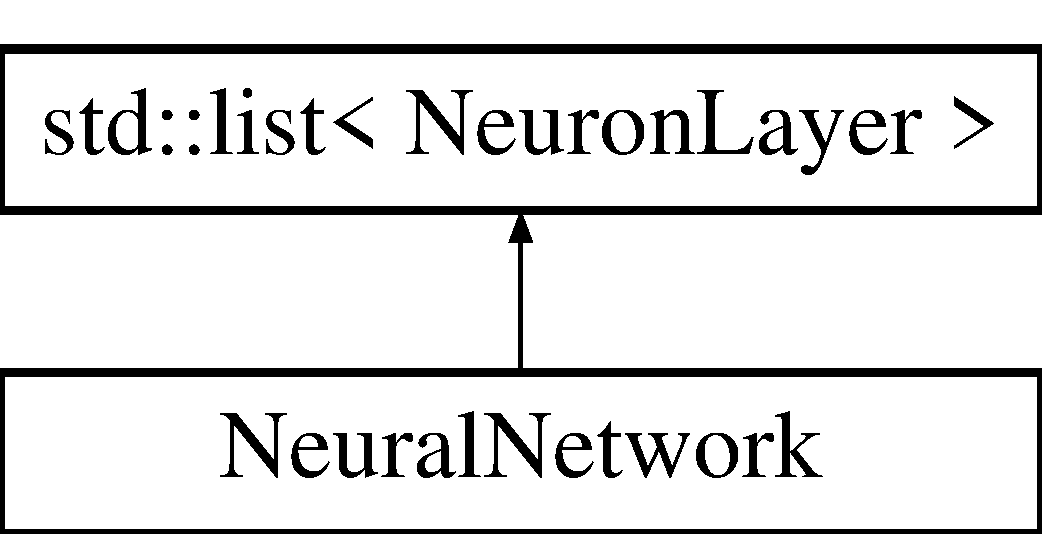
\includegraphics[height=2.000000cm]{classNeuralNetwork}
\end{center}
\end{figure}
\subsection*{Public Types}
\begin{DoxyCompactItemize}
\item 
\mbox{\Hypertarget{classNeuralNetwork_a31de381df65f261fd0f38e0559995d1a}\label{classNeuralNetwork_a31de381df65f261fd0f38e0559995d1a}} 
using {\bfseries Ptr} = std\+::shared\+\_\+ptr$<$ \hyperlink{classNeuralNetwork}{Neural\+Network} $>$
\end{DoxyCompactItemize}
\subsection*{Public Member Functions}
\begin{DoxyCompactItemize}
\item 
\mbox{\Hypertarget{classNeuralNetwork_accce4a7728e89a009a9d4ca1758c9b9d}\label{classNeuralNetwork_accce4a7728e89a009a9d4ca1758c9b9d}} 
\hyperlink{classNeuralNetwork_accce4a7728e89a009a9d4ca1758c9b9d}{Neural\+Network} ()
\begin{DoxyCompactList}\small\item\em Constructeur permettant d\textquotesingle{}initialiser une réseau neuronal vide. \end{DoxyCompactList}\item 
\hyperlink{classNeuralNetwork_a85cd20f411e96dfd28954fcda39badb7}{Neural\+Network} (std\+::vector$<$ unsigned int $>$ layer\+Sizes, std\+::vector$<$ Functions\+::\+Activation\+Fun $>$ activation\+Funs)
\begin{DoxyCompactList}\small\item\em Constructeur permettant d\textquotesingle{}initialiser un réseau neuronal avec choix des fonctions d\textquotesingle{}activation. \end{DoxyCompactList}\item 
\hyperlink{classNeuralNetwork_ab4015471a72a3d00b6bcabf156526f7b}{Neural\+Network} (std\+::vector$<$ unsigned int $>$ layer\+Sizes)
\begin{DoxyCompactList}\small\item\em Constructeur permettant d\textquotesingle{}initialiser un réseau neuronal avec la fonction par défaut. \end{DoxyCompactList}\item 
{\footnotesize template$<$typename Container $>$ }\\\hyperlink{classNeuralNetwork_a7943bb4e9cb96aae048b236d4f1dd979}{Neural\+Network} (Container layer\+List)
\begin{DoxyCompactList}\small\item\em Constructeur permettant d\textquotesingle{}initialiser le réseau neuronal avec un conteneur (vector, list...) de neuron\+Layer. \end{DoxyCompactList}\item 
\mbox{\Hypertarget{classNeuralNetwork_a98cab3b3726fbf06dca316068c29c783}\label{classNeuralNetwork_a98cab3b3726fbf06dca316068c29c783}} 
Eigen\+::\+Vector\+Xf {\bfseries process} (Eigen\+::\+Vector\+Xf input)
\end{DoxyCompactItemize}
\subsection*{Friends}
\begin{DoxyCompactItemize}
\item 
std\+::ostream \& \hyperlink{classNeuralNetwork_a0ecebf9a494437efb917804ed271e13f}{operator$<$$<$} (std\+::ostream \&flux, \hyperlink{classNeuralNetwork}{Neural\+Network} network)
\begin{DoxyCompactList}\small\item\em Fonction utilitaire permettant d\textquotesingle{}afficher le réseau de neurones. \end{DoxyCompactList}\end{DoxyCompactItemize}


\subsection{Constructor \& Destructor Documentation}
\mbox{\Hypertarget{classNeuralNetwork_a85cd20f411e96dfd28954fcda39badb7}\label{classNeuralNetwork_a85cd20f411e96dfd28954fcda39badb7}} 
\index{Neural\+Network@{Neural\+Network}!Neural\+Network@{Neural\+Network}}
\index{Neural\+Network@{Neural\+Network}!Neural\+Network@{Neural\+Network}}
\subsubsection{\texorpdfstring{Neural\+Network()}{NeuralNetwork()}\hspace{0.1cm}{\footnotesize\ttfamily [1/3]}}
{\footnotesize\ttfamily Neural\+Network\+::\+Neural\+Network (\begin{DoxyParamCaption}\item[{std\+::vector$<$ unsigned int $>$}]{layer\+Sizes,  }\item[{std\+::vector$<$ Functions\+::\+Activation\+Fun $>$}]{activation\+Funs }\end{DoxyParamCaption})}



Constructeur permettant d\textquotesingle{}initialiser un réseau neuronal avec choix des fonctions d\textquotesingle{}activation. 

Constructeur permettant l\textquotesingle{}initialisation d\textquotesingle{}un réseau à n couches à partir des (n+1) tailles d\textquotesingle{}input/output (la sortie d\textquotesingle{}une couche est l\textquotesingle{}entrée de la suivante), avec choix des fonctions d\textquotesingle{}activation 
\begin{DoxyParams}{Parameters}
{\em layer\+Sizes} & les tailles des vecteurs d\textquotesingle{}entrées/sorties \\
\hline
{\em activation\+Funs} & le vector contenant les fonctions d\textquotesingle{}activation de chaque couche \\
\hline
\end{DoxyParams}
\mbox{\Hypertarget{classNeuralNetwork_ab4015471a72a3d00b6bcabf156526f7b}\label{classNeuralNetwork_ab4015471a72a3d00b6bcabf156526f7b}} 
\index{Neural\+Network@{Neural\+Network}!Neural\+Network@{Neural\+Network}}
\index{Neural\+Network@{Neural\+Network}!Neural\+Network@{Neural\+Network}}
\subsubsection{\texorpdfstring{Neural\+Network()}{NeuralNetwork()}\hspace{0.1cm}{\footnotesize\ttfamily [2/3]}}
{\footnotesize\ttfamily Neural\+Network\+::\+Neural\+Network (\begin{DoxyParamCaption}\item[{std\+::vector$<$ unsigned int $>$}]{layer\+Sizes }\end{DoxyParamCaption})}



Constructeur permettant d\textquotesingle{}initialiser un réseau neuronal avec la fonction par défaut. 

Constructeur permettant l\textquotesingle{}initialisation d\textquotesingle{}un réseau à n couches à partir des (n+1) tailles d\textquotesingle{}input/output (la sortie d\textquotesingle{}une couche est l\textquotesingle{}entrée de la suivante). La fonction d\textquotesingle{}activation choisie est la fonction d\textquotesingle{}activation par défaut 
\begin{DoxyParams}{Parameters}
{\em layer\+Sizes} & les tailles des vecteurs d\textquotesingle{}entrées/sorties \\
\hline
\end{DoxyParams}
\mbox{\Hypertarget{classNeuralNetwork_a7943bb4e9cb96aae048b236d4f1dd979}\label{classNeuralNetwork_a7943bb4e9cb96aae048b236d4f1dd979}} 
\index{Neural\+Network@{Neural\+Network}!Neural\+Network@{Neural\+Network}}
\index{Neural\+Network@{Neural\+Network}!Neural\+Network@{Neural\+Network}}
\subsubsection{\texorpdfstring{Neural\+Network()}{NeuralNetwork()}\hspace{0.1cm}{\footnotesize\ttfamily [3/3]}}
{\footnotesize\ttfamily template$<$typename Container $>$ \\
Neural\+Network\+::\+Neural\+Network (\begin{DoxyParamCaption}\item[{Container}]{layer\+List }\end{DoxyParamCaption})}



Constructeur permettant d\textquotesingle{}initialiser le réseau neuronal avec un conteneur (vector, list...) de neuron\+Layer. 


\begin{DoxyParams}{Parameters}
{\em layer\+List} & la liste des couches de neurones \\
\hline
\end{DoxyParams}


\subsection{Friends And Related Function Documentation}
\mbox{\Hypertarget{classNeuralNetwork_a0ecebf9a494437efb917804ed271e13f}\label{classNeuralNetwork_a0ecebf9a494437efb917804ed271e13f}} 
\index{Neural\+Network@{Neural\+Network}!operator$<$$<$@{operator$<$$<$}}
\index{operator$<$$<$@{operator$<$$<$}!Neural\+Network@{Neural\+Network}}
\subsubsection{\texorpdfstring{operator$<$$<$}{operator<<}}
{\footnotesize\ttfamily std\+::ostream\& operator$<$$<$ (\begin{DoxyParamCaption}\item[{std\+::ostream \&}]{flux,  }\item[{\hyperlink{classNeuralNetwork}{Neural\+Network}}]{network }\end{DoxyParamCaption})\hspace{0.3cm}{\ttfamily [friend]}}



Fonction utilitaire permettant d\textquotesingle{}afficher le réseau de neurones. 

Cette fonction affiche les matrices de poids des différents layers du réseau 

The documentation for this class was generated from the following files\+:\begin{DoxyCompactItemize}
\item 
headers/neuralnetwork.\+hpp\item 
headers/neuralnetwork.\+inl\item 
sources/neuralnetwork.\+cpp\end{DoxyCompactItemize}

\hypertarget{classNeuronLayer}{}\section{Neuron\+Layer Class Reference}
\label{classNeuronLayer}\index{Neuron\+Layer@{Neuron\+Layer}}


Classe modélisant une couche de neurones.  




{\ttfamily \#include $<$neuronlayer.\+hpp$>$}



Collaboration diagram for Neuron\+Layer\+:\nopagebreak
\begin{figure}[H]
\begin{center}
\leavevmode
\includegraphics[width=204pt]{classNeuronLayer__coll__graph}
\end{center}
\end{figure}
\subsection*{Public Member Functions}
\begin{DoxyCompactItemize}
\item 
\hyperlink{classNeuronLayer_afe2804871685b8103d7cd461460e7b31}{Neuron\+Layer} (unsigned int input\+Size, unsigned int output\+Size, std\+::function$<$ float(float)$>$ activationF=\hyperlink{structFunctions_a773de9cd59f7ccc3e2fe9822f0536ae4}{Functions\+::sigmoid}(10.f))
\begin{DoxyCompactList}\small\item\em Constructeur permettant d\textquotesingle{}initialiser les paramètres de la couche de neurones. \end{DoxyCompactList}\item 
Eigen\+::\+Vector\+Xf \hyperlink{classNeuronLayer_aa374ba7d040ae618b5037aa88e5efae7}{process} (Eigen\+::\+Vector\+Xf inputs)
\begin{DoxyCompactList}\small\item\em La fonction effectuant le calcul de la sortie en fonction de l\textquotesingle{}entrée. \end{DoxyCompactList}\item 
Eigen\+::\+Vector\+Xf \hyperlink{classNeuronLayer_a0896580aa265681f77efbcb81c6c8150}{back\+Prop} (Eigen\+::\+Vector\+Xf xn\+Partial\+Derivative, float step)
\begin{DoxyCompactList}\small\item\em La fonction effectuant les calculs de rétropropagation. \end{DoxyCompactList}\item 
void \hyperlink{classNeuronLayer_af4f8a2ea263ab0c242124571db916d73}{reset} ()
\end{DoxyCompactItemize}
\subsection*{Private Member Functions}
\begin{DoxyCompactItemize}
\item 
Eigen\+::\+Matrix\+Xf \hyperlink{classNeuronLayer_a8b4572b9b3cd779233f8c269c3eca608}{fn\+Derivative\+Matrix} () const
\begin{DoxyCompactList}\small\item\em Fonction renvoyant le vecteur des dérivées de Fn évalué en Yn. \end{DoxyCompactList}\end{DoxyCompactItemize}
\subsection*{Private Attributes}
\begin{DoxyCompactItemize}
\item 
Eigen\+::\+Matrix\+Xf \hyperlink{classNeuronLayer_ab6aaf5dc22c97ba46db5ac5e8715ed8f}{m\+Poids}
\begin{DoxyCompactList}\small\item\em La matrice des poids de la couche de neurones. \end{DoxyCompactList}\item 
Eigen\+::\+Vector\+Xf \hyperlink{classNeuronLayer_a6d1c0d70051d87dace0cdf654d866a4a}{m\+Biais}
\begin{DoxyCompactList}\small\item\em La matrice des biais de la couche de neurones. \end{DoxyCompactList}\item 
std\+::function$<$ float(float)$>$ \hyperlink{classNeuronLayer_ac0ff52b79f1a068e75f0eb0309b5e683}{m\+Activation\+Fun}
\begin{DoxyCompactList}\small\item\em La fonction d\textquotesingle{}activation de la couche de neurones. \end{DoxyCompactList}\item 
Eigen\+::\+Vector\+Xf \hyperlink{classNeuronLayer_a5b5ccadbab1d38fd3b09fcab7dc01148}{m\+Buffer\+Activation\+Level}
\begin{DoxyCompactList}\small\item\em Buffer pour stocker Yn = Wn\+Xn-\/1, nécessaire pour la backprop. \end{DoxyCompactList}\item 
Eigen\+::\+Vector\+Xf \hyperlink{classNeuronLayer_ab5a3fc010c33628e37b5a19d370978e9}{m\+Buffer\+Input}
\begin{DoxyCompactList}\small\item\em Buffer pour stocker l\textquotesingle{}input, nécessaire pour la backrprop. \end{DoxyCompactList}\end{DoxyCompactItemize}
\subsection*{Friends}
\begin{DoxyCompactItemize}
\item 
std\+::ostream \& \hyperlink{classNeuronLayer_adbe40702c22550c0392b3447e5d63c9a}{operator$<$$<$} (std\+::ostream \&flux, \hyperlink{classNeuronLayer}{Neuron\+Layer} nl)
\begin{DoxyCompactList}\small\item\em Fonction utilitaire permettant d\textquotesingle{}afficher le neurone. \end{DoxyCompactList}\end{DoxyCompactItemize}


\subsection{Detailed Description}
Classe modélisant une couche de neurones. 

Neurone\+Layer représente une couche de neurones, avec une matrice de poids et une fonction d\textquotesingle{}activation 

\subsection{Constructor \& Destructor Documentation}
\mbox{\Hypertarget{classNeuronLayer_afe2804871685b8103d7cd461460e7b31}\label{classNeuronLayer_afe2804871685b8103d7cd461460e7b31}} 
\index{Neuron\+Layer@{Neuron\+Layer}!Neuron\+Layer@{Neuron\+Layer}}
\index{Neuron\+Layer@{Neuron\+Layer}!Neuron\+Layer@{Neuron\+Layer}}
\subsubsection{\texorpdfstring{Neuron\+Layer()}{NeuronLayer()}}
{\footnotesize\ttfamily Neuron\+Layer\+::\+Neuron\+Layer (\begin{DoxyParamCaption}\item[{unsigned int}]{input\+Size,  }\item[{unsigned int}]{output\+Size,  }\item[{std\+::function$<$ float(float)$>$}]{activationF = {\ttfamily \hyperlink{structFunctions_a773de9cd59f7ccc3e2fe9822f0536ae4}{Functions\+::sigmoid}(10.f)} }\end{DoxyParamCaption})}



Constructeur permettant d\textquotesingle{}initialiser les paramètres de la couche de neurones. 


\begin{DoxyParams}{Parameters}
{\em input\+Size} & le nombre d\textquotesingle{}inputs de cette couche \\
\hline
{\em output\+Size} & le nombre d\textquotesingle{}outputs de cette couche \\
\hline
{\em activationF} & la fonction d\textquotesingle{}activation de tous les neurones de la couche\\
\hline
\end{DoxyParams}
La matrice de poids est de dimension output\+Size x input\+Size 

\subsection{Member Function Documentation}
\mbox{\Hypertarget{classNeuronLayer_a0896580aa265681f77efbcb81c6c8150}\label{classNeuronLayer_a0896580aa265681f77efbcb81c6c8150}} 
\index{Neuron\+Layer@{Neuron\+Layer}!back\+Prop@{back\+Prop}}
\index{back\+Prop@{back\+Prop}!Neuron\+Layer@{Neuron\+Layer}}
\subsubsection{\texorpdfstring{back\+Prop()}{backProp()}}
{\footnotesize\ttfamily Eigen\+::\+Vector\+Xf Neuron\+Layer\+::back\+Prop (\begin{DoxyParamCaption}\item[{Eigen\+::\+Vector\+Xf}]{xn\+Partial\+Derivative,  }\item[{float}]{step }\end{DoxyParamCaption})}



La fonction effectuant les calculs de rétropropagation. 

La fonction calcule les 3 équations matricielles, mets à jour les poids et renvoie le vecteur de dérivées partielles nécessaires pour la backprop de la couche précédente 
\begin{DoxyParams}{Parameters}
{\em xn\+Partial\+Derivative} & le vecteur des dérivées partielles selon Xn \\
\hline
{\em step} & le pas d\textquotesingle{}apprentissage \\
\hline
\end{DoxyParams}
\begin{DoxyReturn}{Returns}
le vecteur des dérivées partielles selon Xn-\/1 à envoyer à la couche précédente 
\end{DoxyReturn}
\mbox{\Hypertarget{classNeuronLayer_a8b4572b9b3cd779233f8c269c3eca608}\label{classNeuronLayer_a8b4572b9b3cd779233f8c269c3eca608}} 
\index{Neuron\+Layer@{Neuron\+Layer}!fn\+Derivative\+Matrix@{fn\+Derivative\+Matrix}}
\index{fn\+Derivative\+Matrix@{fn\+Derivative\+Matrix}!Neuron\+Layer@{Neuron\+Layer}}
\subsubsection{\texorpdfstring{fn\+Derivative\+Matrix()}{fnDerivativeMatrix()}}
{\footnotesize\ttfamily Eigen\+::\+Matrix\+Xf Neuron\+Layer\+::fn\+Derivative\+Matrix (\begin{DoxyParamCaption}{ }\end{DoxyParamCaption}) const\hspace{0.3cm}{\ttfamily [private]}}



Fonction renvoyant le vecteur des dérivées de Fn évalué en Yn. 

Cette fonction calcule Fn\textquotesingle{}(Yn) ou Yn = m\+Buffer\+Activation\+Level \begin{DoxyReturn}{Returns}
le vecteur des dérivées mises en colonne 
\end{DoxyReturn}
\mbox{\Hypertarget{classNeuronLayer_aa374ba7d040ae618b5037aa88e5efae7}\label{classNeuronLayer_aa374ba7d040ae618b5037aa88e5efae7}} 
\index{Neuron\+Layer@{Neuron\+Layer}!process@{process}}
\index{process@{process}!Neuron\+Layer@{Neuron\+Layer}}
\subsubsection{\texorpdfstring{process()}{process()}}
{\footnotesize\ttfamily Eigen\+::\+Vector\+Xf Neuron\+Layer\+::process (\begin{DoxyParamCaption}\item[{Eigen\+::\+Vector\+Xf}]{inputs }\end{DoxyParamCaption})}



La fonction effectuant le calcul de la sortie en fonction de l\textquotesingle{}entrée. 


\begin{DoxyParams}{Parameters}
{\em inputs} & le vecteur d\textquotesingle{}input de la couche de neurones \\
\hline
\end{DoxyParams}
\begin{DoxyReturn}{Returns}
le vecteur d\textquotesingle{}output de la couche de neurones la fonction effectue le produit matriciel des poids par les entrées, puis applique la fonction d\textquotesingle{}activation 
\end{DoxyReturn}
\mbox{\Hypertarget{classNeuronLayer_af4f8a2ea263ab0c242124571db916d73}\label{classNeuronLayer_af4f8a2ea263ab0c242124571db916d73}} 
\index{Neuron\+Layer@{Neuron\+Layer}!reset@{reset}}
\index{reset@{reset}!Neuron\+Layer@{Neuron\+Layer}}
\subsubsection{\texorpdfstring{reset()}{reset()}}
{\footnotesize\ttfamily void Neuron\+Layer\+::reset (\begin{DoxyParamCaption}{ }\end{DoxyParamCaption})}



\subsection{Friends And Related Function Documentation}
\mbox{\Hypertarget{classNeuronLayer_adbe40702c22550c0392b3447e5d63c9a}\label{classNeuronLayer_adbe40702c22550c0392b3447e5d63c9a}} 
\index{Neuron\+Layer@{Neuron\+Layer}!operator$<$$<$@{operator$<$$<$}}
\index{operator$<$$<$@{operator$<$$<$}!Neuron\+Layer@{Neuron\+Layer}}
\subsubsection{\texorpdfstring{operator$<$$<$}{operator<<}}
{\footnotesize\ttfamily std\+::ostream\& operator$<$$<$ (\begin{DoxyParamCaption}\item[{std\+::ostream \&}]{flux,  }\item[{\hyperlink{classNeuronLayer}{Neuron\+Layer}}]{nl }\end{DoxyParamCaption})\hspace{0.3cm}{\ttfamily [friend]}}



Fonction utilitaire permettant d\textquotesingle{}afficher le neurone. 

Cette fonction affiche la matrice des poids 

\subsection{Field Documentation}
\mbox{\Hypertarget{classNeuronLayer_ac0ff52b79f1a068e75f0eb0309b5e683}\label{classNeuronLayer_ac0ff52b79f1a068e75f0eb0309b5e683}} 
\index{Neuron\+Layer@{Neuron\+Layer}!m\+Activation\+Fun@{m\+Activation\+Fun}}
\index{m\+Activation\+Fun@{m\+Activation\+Fun}!Neuron\+Layer@{Neuron\+Layer}}
\subsubsection{\texorpdfstring{m\+Activation\+Fun}{mActivationFun}}
{\footnotesize\ttfamily std\+::function$<$float(float)$>$ Neuron\+Layer\+::m\+Activation\+Fun\hspace{0.3cm}{\ttfamily [private]}}



La fonction d\textquotesingle{}activation de la couche de neurones. 

\mbox{\Hypertarget{classNeuronLayer_a6d1c0d70051d87dace0cdf654d866a4a}\label{classNeuronLayer_a6d1c0d70051d87dace0cdf654d866a4a}} 
\index{Neuron\+Layer@{Neuron\+Layer}!m\+Biais@{m\+Biais}}
\index{m\+Biais@{m\+Biais}!Neuron\+Layer@{Neuron\+Layer}}
\subsubsection{\texorpdfstring{m\+Biais}{mBiais}}
{\footnotesize\ttfamily Eigen\+::\+Vector\+Xf Neuron\+Layer\+::m\+Biais\hspace{0.3cm}{\ttfamily [private]}}



La matrice des biais de la couche de neurones. 

\mbox{\Hypertarget{classNeuronLayer_a5b5ccadbab1d38fd3b09fcab7dc01148}\label{classNeuronLayer_a5b5ccadbab1d38fd3b09fcab7dc01148}} 
\index{Neuron\+Layer@{Neuron\+Layer}!m\+Buffer\+Activation\+Level@{m\+Buffer\+Activation\+Level}}
\index{m\+Buffer\+Activation\+Level@{m\+Buffer\+Activation\+Level}!Neuron\+Layer@{Neuron\+Layer}}
\subsubsection{\texorpdfstring{m\+Buffer\+Activation\+Level}{mBufferActivationLevel}}
{\footnotesize\ttfamily Eigen\+::\+Vector\+Xf Neuron\+Layer\+::m\+Buffer\+Activation\+Level\hspace{0.3cm}{\ttfamily [private]}}



Buffer pour stocker Yn = Wn\+Xn-\/1, nécessaire pour la backprop. 

\mbox{\Hypertarget{classNeuronLayer_ab5a3fc010c33628e37b5a19d370978e9}\label{classNeuronLayer_ab5a3fc010c33628e37b5a19d370978e9}} 
\index{Neuron\+Layer@{Neuron\+Layer}!m\+Buffer\+Input@{m\+Buffer\+Input}}
\index{m\+Buffer\+Input@{m\+Buffer\+Input}!Neuron\+Layer@{Neuron\+Layer}}
\subsubsection{\texorpdfstring{m\+Buffer\+Input}{mBufferInput}}
{\footnotesize\ttfamily Eigen\+::\+Vector\+Xf Neuron\+Layer\+::m\+Buffer\+Input\hspace{0.3cm}{\ttfamily [private]}}



Buffer pour stocker l\textquotesingle{}input, nécessaire pour la backrprop. 

\mbox{\Hypertarget{classNeuronLayer_ab6aaf5dc22c97ba46db5ac5e8715ed8f}\label{classNeuronLayer_ab6aaf5dc22c97ba46db5ac5e8715ed8f}} 
\index{Neuron\+Layer@{Neuron\+Layer}!m\+Poids@{m\+Poids}}
\index{m\+Poids@{m\+Poids}!Neuron\+Layer@{Neuron\+Layer}}
\subsubsection{\texorpdfstring{m\+Poids}{mPoids}}
{\footnotesize\ttfamily Eigen\+::\+Matrix\+Xf Neuron\+Layer\+::m\+Poids\hspace{0.3cm}{\ttfamily [private]}}



La matrice des poids de la couche de neurones. 



The documentation for this class was generated from the following files\+:\begin{DoxyCompactItemize}
\item 
headers/\hyperlink{neuronlayer_8hpp}{neuronlayer.\+hpp}\item 
sources/\hyperlink{neuronlayer_8cpp}{neuronlayer.\+cpp}\end{DoxyCompactItemize}

\hypertarget{classStatistics}{}\section{Statistics Class Reference}
\label{classStatistics}\index{Statistics@{Statistics}}


Classe statique utile pour les calculs statistiques.  




{\ttfamily \#include $<$utility.\+hpp$>$}



Collaboration diagram for Statistics\+:\nopagebreak
\begin{figure}[H]
\begin{center}
\leavevmode
\includegraphics[width=178pt]{classStatistics__coll__graph}
\end{center}
\end{figure}
\subsection*{Data Structures}
\begin{DoxyCompactItemize}
\item 
struct \hyperlink{structStatistics_1_1Data}{Data}
\begin{DoxyCompactList}\small\item\em Structure contenant les mesures d\textquotesingle{}un jeu de donnée. \end{DoxyCompactList}\end{DoxyCompactItemize}
\subsection*{Static Public Member Functions}
\begin{DoxyCompactItemize}
\item 
static \hyperlink{structStatistics_1_1Data}{Data} \hyperlink{classStatistics_aaa2152a3f262ce8d003663f993420c4c}{process\+Data} (const std\+::vector$<$ float $>$ \&data\+Vect)
\begin{DoxyCompactList}\small\item\em Fonction calculant les moyennes, écarts-\/types et les données associées du jeu de données. \end{DoxyCompactList}\item 
static float \hyperlink{classStatistics_ae1c12077162711aa0ea8b4ee6e15b4da}{process\+Median} (std\+::vector$<$ float $>$ data\+Vect)
\begin{DoxyCompactList}\small\item\em Fonction calculant la médiane d\textquotesingle{}un jeu de données. \end{DoxyCompactList}\end{DoxyCompactItemize}


\subsection{Detailed Description}
Classe statique utile pour les calculs statistiques. 

\subsection{Member Function Documentation}
\mbox{\Hypertarget{classStatistics_aaa2152a3f262ce8d003663f993420c4c}\label{classStatistics_aaa2152a3f262ce8d003663f993420c4c}} 
\index{Statistics@{Statistics}!process\+Data@{process\+Data}}
\index{process\+Data@{process\+Data}!Statistics@{Statistics}}
\subsubsection{\texorpdfstring{process\+Data()}{processData()}}
{\footnotesize\ttfamily \hyperlink{structStatistics_1_1Data}{Statistics\+::\+Data} Statistics\+::process\+Data (\begin{DoxyParamCaption}\item[{const std\+::vector$<$ float $>$ \&}]{data\+Vect }\end{DoxyParamCaption})\hspace{0.3cm}{\ttfamily [static]}}



Fonction calculant les moyennes, écarts-\/types et les données associées du jeu de données. 

Calcul de la moyenne et de l\textquotesingle{}intervalle de confiance Calcul de l\textquotesingle{}écart-\/type et de son intervalle de confiance 
\begin{DoxyParams}{Parameters}
{\em data\+Vect} & Vecteur de données \\
\hline
\end{DoxyParams}
\mbox{\Hypertarget{classStatistics_ae1c12077162711aa0ea8b4ee6e15b4da}\label{classStatistics_ae1c12077162711aa0ea8b4ee6e15b4da}} 
\index{Statistics@{Statistics}!process\+Median@{process\+Median}}
\index{process\+Median@{process\+Median}!Statistics@{Statistics}}
\subsubsection{\texorpdfstring{process\+Median()}{processMedian()}}
{\footnotesize\ttfamily float Statistics\+::process\+Median (\begin{DoxyParamCaption}\item[{std\+::vector$<$ float $>$}]{data\+Vect }\end{DoxyParamCaption})\hspace{0.3cm}{\ttfamily [static]}}



Fonction calculant la médiane d\textquotesingle{}un jeu de données. 


\begin{DoxyParams}{Parameters}
{\em data\+Vect} & Vecteur de données \\
\hline
\end{DoxyParams}


The documentation for this class was generated from the following files\+:\begin{DoxyCompactItemize}
\item 
headers/\hyperlink{utility_8hpp}{utility.\+hpp}\item 
sources/\hyperlink{utility_8cpp}{utility.\+cpp}\end{DoxyCompactItemize}

\hypertarget{classTeacher}{}\section{Teacher Class Reference}
\label{classTeacher}\index{Teacher@{Teacher}}
\subsection*{Public Member Functions}
\begin{DoxyCompactItemize}
\item 
\hyperlink{classTeacher_a8ca95fc7a29e082a676d420b9fd8fd67}{Teacher} (Neural\+Network\+::\+Ptr network)
\begin{DoxyCompactList}\small\item\em Constructeur par unique pointer. \end{DoxyCompactList}\item 
\hyperlink{classTeacher_afd32ab70242f2c5886d030a5e7d05919}{Teacher} (\hyperlink{classNeuralNetwork}{Neural\+Network} $\ast$network)
\begin{DoxyCompactList}\small\item\em Constructeur par pointer. \end{DoxyCompactList}\item 
void \hyperlink{classTeacher_a99fc69c5319be890394d2c8503e217c8}{back\+Prop} (Eigen\+::\+Vector\+Xf input, Eigen\+::\+Vector\+Xf desired\+Output, float step=0.\+2, float dx=0.\+05)
\begin{DoxyCompactList}\small\item\em Fonction appliquant la méthode de rétropropagation sur m\+Network. \end{DoxyCompactList}\end{DoxyCompactItemize}


\subsection{Constructor \& Destructor Documentation}
\mbox{\Hypertarget{classTeacher_a8ca95fc7a29e082a676d420b9fd8fd67}\label{classTeacher_a8ca95fc7a29e082a676d420b9fd8fd67}} 
\index{Teacher@{Teacher}!Teacher@{Teacher}}
\index{Teacher@{Teacher}!Teacher@{Teacher}}
\subsubsection{\texorpdfstring{Teacher()}{Teacher()}\hspace{0.1cm}{\footnotesize\ttfamily [1/2]}}
{\footnotesize\ttfamily Teacher\+::\+Teacher (\begin{DoxyParamCaption}\item[{Neural\+Network\+::\+Ptr}]{network }\end{DoxyParamCaption})}



Constructeur par unique pointer. 

Construit un teacher supervisant l\textquotesingle{}apprentissage d\textquotesingle{}un réseau de neurone 
\begin{DoxyParams}{Parameters}
{\em network} & un smart pointeur sur le réseau dont on veut superviser l\textquotesingle{}apprentissage \\
\hline
\end{DoxyParams}
\mbox{\Hypertarget{classTeacher_afd32ab70242f2c5886d030a5e7d05919}\label{classTeacher_afd32ab70242f2c5886d030a5e7d05919}} 
\index{Teacher@{Teacher}!Teacher@{Teacher}}
\index{Teacher@{Teacher}!Teacher@{Teacher}}
\subsubsection{\texorpdfstring{Teacher()}{Teacher()}\hspace{0.1cm}{\footnotesize\ttfamily [2/2]}}
{\footnotesize\ttfamily Teacher\+::\+Teacher (\begin{DoxyParamCaption}\item[{\hyperlink{classNeuralNetwork}{Neural\+Network} $\ast$}]{network }\end{DoxyParamCaption})}



Constructeur par pointer. 

Construit un teacher supervisant l\textquotesingle{}apprentissage d\textquotesingle{}un réseau de neurone 
\begin{DoxyParams}{Parameters}
{\em network} & un pointeur sur le réseau dont on veut superviser l\textquotesingle{}apprentissage \\
\hline
\end{DoxyParams}


\subsection{Member Function Documentation}
\mbox{\Hypertarget{classTeacher_a99fc69c5319be890394d2c8503e217c8}\label{classTeacher_a99fc69c5319be890394d2c8503e217c8}} 
\index{Teacher@{Teacher}!back\+Prop@{back\+Prop}}
\index{back\+Prop@{back\+Prop}!Teacher@{Teacher}}
\subsubsection{\texorpdfstring{back\+Prop()}{backProp()}}
{\footnotesize\ttfamily void Teacher\+::back\+Prop (\begin{DoxyParamCaption}\item[{Eigen\+::\+Vector\+Xf}]{input,  }\item[{Eigen\+::\+Vector\+Xf}]{desired\+Output,  }\item[{float}]{step = {\ttfamily 0.2},  }\item[{float}]{dx = {\ttfamily 0.05} }\end{DoxyParamCaption})}



Fonction appliquant la méthode de rétropropagation sur m\+Network. 

Calcule la première dérivée d\+E/d\+Xn puis propage l\textquotesingle{}erreur à travers le réseau 
\begin{DoxyParams}{Parameters}
{\em input} & le vecteur d\textquotesingle{}input que le réseau va process \\
\hline
{\em desired\+Output} & la sortie modèle dont on veut se rapprocher \\
\hline
{\em step} & le pas d\textquotesingle{}apprentissage \\
\hline
{\em dx} & le deplacement élémentaire pour calculer la dérivée \\
\hline
\end{DoxyParams}


The documentation for this class was generated from the following files\+:\begin{DoxyCompactItemize}
\item 
headers/teacher.\+hpp\item 
sources/teacher.\+cpp\end{DoxyCompactItemize}

%--- End generated contents ---

% Index
\backmatter
\newpage
\phantomsection
\clearemptydoublepage
\addcontentsline{toc}{chapter}{Index}
\printindex

\end{document}
